% !TeX program = lualatex
\documentclass[a4paper,12pt]{article}
\usepackage[margin=2.5cm,headheight=16pt]{geometry}
\usepackage{fontspec}
\usepackage{babel}
\babelprovide[import,main]{chinese}
\babelfont{rm}[ItalicFont={Noto Serif CJK SC}]{Noto Serif CJK SC}
\babelfont{sf}{Noto Sans CJK SC}
\babelfont{tt}{DejaVu Sans Mono}
\newfontfamily\codefont{Noto Sans Mono CJK SC}
\usepackage{amsmath,amssymb,amsthm,booktabs,longtable,array}
\usepackage{xcolor,graphicx,fancyhdr,fancyvrb}
\usepackage[unicode,hidelinks]{hyperref}
\usepackage{listings}
\linespread{1.22}
\setlength{\parindent}{2em}
\setlength{\parskip}{0.25em}
\setlength{\emergencystretch}{3em}
\pagestyle{fancy}\fancyhf{}\fancyfoot[C]{\thepage}
\renewcommand{\headrulewidth}{0pt}
\renewcommand{\figurename}{图}\renewcommand{\tablename}{表}
\renewcommand{\refname}{参考文献}
\theoremstyle{definition}
\newtheorem{proposition}{命题}[section]
\renewcommand{\proofname}{证明}
\newcommand{\R}{\mathbb R}
\newcommand{\norm}[1]{\left\lVert #1\right\rVert}
\newcommand{\disk}{\overline B}
\newcommand{\eps}{\varepsilon}
\newcommand{\ind}{\mathbf 1}
\newcommand{\placeholder}[2]{\begin{figure}[htbp]\centering\fbox{\parbox{0.90\linewidth}{\small [#2]}}\caption{#1}\end{figure}}
\lstset{basicstyle=\codefont\scriptsize,breaklines=true,columns=fullflexible,keepspaces=true,showstringspaces=false,frame=single,numbers=left,numberstyle=\tiny,numbersep=5pt}
\begin{document}
\begin{center}
{\LARGE\bfseries 基于知识矩阵与集合估计的\\[0.25em]无线电干扰源自适应定位与清除}\par
\vspace{1em}{\large\bfseries 摘要}
\end{center}
针对未知数量、位置及发射方向的无线电干扰源定位清除问题，建立知识矩阵、集合估计与覆盖认证相结合的自适应模型，以全部清除为约束，以移动、切频、检测和光学清除的虚拟总耗时为目标。

对问题一，将示向误差区间表示为两个半平面，逐次裁剪形成交会定位区域，利用顶点对距离或旋转卡壳计算直径。通过等边三角形反例说明直径圆未必覆盖区域，并以最小包围圆半径不超过20米作为单点保证清除判据。

对问题二，利用同一源接收半径固定的性质，推导三个1000米圆盘交集构成的稳健接收区域，再用名义交会角筛选候选点。圆心首测、附加均匀先验下的参考选点为沿示向前进850米、横移520米，接收裕量约3.56米；一般首测位置按目标圆重新裁剪，不宣称两次测向必能清除。

对问题三，以频道与路径位置构造知识矩阵，将七点覆盖扫描与已发现目标合并调度，通过最近邻、2-opt及or-opt滚动缩短路线。利用清除失败的20米排除圆和25米方格覆盖，实现直接试清、必要补测和覆盖兜底。最终配置在本地种子61至160的100例中全部清除，每源时间中位数272.08秒；消融表明主要时间收益来自布局与路由调整。

对问题四，证明任意定向半圆被检测点命中等价于源位置处于1000米内检测点的凸包，采用24点联合优化布局，并以递归单元数值证书检验连续域覆盖。以方向无关的光学覆盖修补波束背面及射线误差造成的清除失败。已有混合与全定向压力测试共520例、6684个源全部清除。两场官方演练中，问题三清除14/14个源、239.82秒/源，问题四清除15/15个源、422.64秒/源。演练与正式测试分别记录；覆盖保证以保守域含真值、格心可达及计划完整执行为前提。

\noindent\textbf{关键词：}知识矩阵；集合估计；局部凸包；联合调度；覆盖式清除
\clearpage
\section{问题重述与总体思路}
在半径 $1800\,\mathrm m$ 的圆域内，有若干位置未知、频道互异的干扰源。机器狗从圆心出发，逐次选择检测位置和频道，根据带有 $\pm1^\circ$ 误差的示向度推断目标位置，并在距离目标不超过 $20\,\mathrm m$ 时完成光学定位与清除。任务要求同时控制移动、切换频道、检测及清除产生的时间\cite{problem,protocol}。

问题一要求给出交会多边形的直径算法，并判断相应直径圆能否覆盖区域。问题二要求在已有一次示向读数后选择第二检测点。问题三要求在全向源、数量未知的条件下尽快完成全部清除。问题四加入定向源，本文保留解法位置。

前三问具有递进关系：问题一提供位置不确定性的几何表达；问题二解决信息获取的位置选择；问题三将单目标定位嵌入多目标覆盖和路径规划。模型采用集合估计描述必然性，用附加概率模型比较典型效率，用执行日志评价实际耗时。
\placeholder{总体模型流程}{绘制四个模块：覆盖扫描、按频道更新可行域、选择目标并补测、光学清除；补测模块返回可行域更新，清除后返回目标调度；最右侧为逐频道终止证书。第四问不绘制。}

\section{基本假设与适用范围}
\begin{enumerate}
\item 干扰源位置、频道和有效接收半径在一次任务中保持不变；不同源的频道互异且信号互不影响。这是将多目标观测按频道分解的依据。
\item 采用题设二维平面、直线移动与恒速模型。不另加障碍物、转弯、加减速及仪器姿态调整代价；检测耗时已包含题设天线调整过程。
\item 示向误差严格处于 $[-1^\circ,1^\circ]$，同一地点同一频道的误差固定。确定性分析不要求误差服从某种分布，也不要求不同地点误差独立。
\item 观测与清除反馈遵守题面和通信协议。全向源在接收半径内返回示向或近距反馈；光学清除只由距离决定。收到成功反馈后才将该频道标记为已清除。
\item 为比较问题二候选点的平均性能，额外采用源位置在目标圆内等面积均匀、接收半径在 $[1000,1500]$ 上均匀、不同检测位置角误差独立均匀的参考先验。这些是评价假设，不能作为题面事实或清除保证。
\item 数值计算采用向外包络和容差复核。空集合、退化多边形及浮点计算异常触发检查或重新检测，不能直接解释为目标不存在。
\end{enumerate}
目标数量在10至16之间只能用于一致性检查。清除10个目标并不能证明任务结束；全向源的全域覆盖证书才可排除未发现目标。

\section{符号说明}
\begin{longtable}{>{$}l<{$}p{9.5cm}}
\toprule
\multicolumn{1}{l}{符号}&含义及单位\\\midrule\endhead
\Omega=\disk(0,R_0)&目标圆域，$R_0=1800\,\mathrm m$；$\disk$ 表示闭圆盘\\
G_j,c_j,\rho_j&第 $j$ 个源的位置、频道及固定有效接收半径，$1000\le\rho_j\le1500\,\mathrm m$\\
a,b&接收半径下、上界，分别为1000和1500米\\
S_i,\theta_i&第 $i$ 个检测点与示向度；推导中角度统一用弧度\\
\eps&最大角误差，$\pi/180$\\
e(\theta),e_\perp(\theta)&$(\cos\theta,\sin\theta)$ 及其逆时针旋转 $90^\circ$ 的单位向量\\
W_i,K_j,\widehat K_j&示向楔形、源位置可行集及其保守多边形外包络\\
D(K),C(K),r_*(K)&区域直径、最小包围圆圆心和半径\\
r_{\rm opt},v&光学作用半径 $20\,\mathrm m$，移动速度 $5\,\mathrm{m/s}$\\
\mathcal P_j,\mathcal N_j&频道 $j$ 的有效接收记录与无信号记录集合\\
\mathcal V,\mathcal C&第二检测点的稳健接收区域与进一步筛选的候选区域\\
r_h,h&覆盖扫描环半径；兜底网格边长上界\\
L,N_m,N_s,N_o,N_c&总路程、检测次数、实际切频次数、光学尝试次数、成功清除数\\
T,\bar t,\eta&虚拟总时间、每源平均定位清除时间、清除比例\\
\bottomrule
\end{longtable}
为简化下标，讨论单个源时省略频道编号。二维叉积定义为 $u\times w=u_xw_y-u_yw_x$，$\operatorname{wrap}$ 将角度映射至 $(-\pi,\pi]$。

\section{问题一：交会定位区域及其直径}
\subsection{示向约束的半平面表示}
令 $u_i^-=e(\theta_i-\eps)$、$u_i^+=e(\theta_i+\eps)$。目标位置满足
\begin{equation}
W_i=\{X:u_i^-\times(X-S_i)\ge0,\quad u_i^+\times(X-S_i)\le0\}.
\label{eq:wedge}
\end{equation}
该形式同时保留“位于射线前方”的信息，避免把示向线误当成无方向直线，也不受 $0^\circ$ 与 $360^\circ$ 跨界影响。

仅使用题目交会信息时，定位区域为 $P=\bigcap_iW_i$。若其非空有界，则为凸多边形；若观测方向接近或约束不足，则可能无界，不能强行给出有限直径。结合已知目标圆域与有效接收半径上界，可进一步构造
\begin{equation}
K=\Omega\cap\bigcap_i\bigl(W_i\cap\disk(S_i,b)\bigr).
\label{eq:region}
\end{equation}
这是含圆弧边界的凸集。计算时将每个圆盘换为外接正 $m$ 边形，得到 $K\subseteq\widehat K$；因此所得直径是精确集合直径的上界。题目给定多边形的直径与这一外包络直径应分别标注。

\subsection{区域构造和直径算法}
若多边形顶点已知，直接计算其凸包后求直径即可。若输入为示向度，按式\eqref{eq:wedge}进行半平面求交；需要圆域约束时，从目标圆的外接多边形开始逐次裁剪。设保留半平面为 $f(X)=n\cdot X+c\ge0$，边端点 $A,B$ 分居两侧，则交点为
\begin{equation}
I=A+\frac{f(A)}{f(A)-f(B)}(B-A).
\label{eq:clip}
\end{equation}
顺次保留域内顶点并补充交点，即得到下一轮多边形。

设最终顶点按逆时针顺序为 $V_1,\ldots,V_m$，则
\begin{equation}
D(P)=\max_{1\le i,j\le m}\norm{V_i-V_j}.
\label{eq:diameter}
\end{equation}
证明见附录。枚举顶点对的时间复杂度为 $O(m^2)$，便于核验；凸多边形可用旋转卡壳枚举对踵点，将该步骤降为 $O(m)$。对每条边推进使三角形面积最大的对侧顶点，在面积相等时同时检查相邻对踵点，避免漏掉平行边情形。一般半平面求交可在排序后用双端队列完成，总体复杂度 $O(n\log n)$；当前逐边裁剪适合边数较少的在线更新。

空集应报告约束不一致；单点直径为零；线段直径为端点距离；无界区域直径为无穷。几何程序把少于三个顶点直接判空的实现方式，需要在最终版本中与这些退化情况分开处理。

\subsection{直径圆不一定覆盖定位区域}
取一对直径端点 $A,B$，令 $M=(A+B)/2$。其直径圆覆盖 $P$ 当且仅当
\begin{equation}
\max_k(V_k-A)\cdot(V_k-B)\le0,
\label{eq:diametercircle}
\end{equation}
因为 $(X-A)\cdot(X-B)=\norm{X-M}^2-D^2/4$，且圆盘是凸集，检查全部顶点即可。

边长为 $D$ 的等边三角形构成反例：最小包围圆半径为 $D/\sqrt3>D/2$，任何直径为 $D$ 的圆都无法覆盖它。对于有限次窄楔形交会，也不能据此假定总有覆盖性；可在三角形各边延长线上放置足够远的楔形顶点，使一条边界沿该边，另一条边界在三角形外侧，三组楔形即可保留这个反例。

一般非空紧平面集满足
\begin{equation}
\frac{D(K)}2\le r_*(K)\le\frac{D(K)}{\sqrt3},\qquad
\text{直径圆可覆盖}\ \Longleftrightarrow\ r_*(K)=\frac{D(K)}2.
\label{eq:jung}
\end{equation}
最小包围圆由两个对径支撑点或三个非共线支撑点确定。可用随机增量算法计算，期望时间为 $O(m)$；最后逐顶点核验，并取实际最大顶点距离作为认证半径。

因此，$D\le40\,\mathrm m$ 只是可用一个20米圆覆盖的必要条件，$D\le20\sqrt3\,\mathrm m$ 是充分条件；直接计算 $r_*\le20\,\mathrm m$ 才是准确判据。若使用外包络 $\widehat K$，该判据仍然充分，但可能偏保守。
\placeholder{直径圆与最小包围圆的区别}{并列绘制一个平行四边形与一个等边三角形。标出直径端点、直径圆圆心、半径；三角形第三顶点落在直径圆外，再画其外接圆。注明示意图不按实际距离比例。}

\section{问题二：第二检测点的选择}
\subsection{第一读数给出的信息}
已有检测点 $S_1$ 和示向度 $\theta_1$，定义
\begin{equation}
A_1=\Omega\cap W_1\cap\disk(S_1,b),\qquad
S_2=S_1+x e(\theta_1)+y e_\perp(\theta_1).
\end{equation}
严格的示向反馈还排除 $\norm{G-S_1}\le5$ 的部分。为保持凸性，稳健几何模型可保留这一小区域作为保守外包络；概率计算则应排除它，或明确说明作了近似。

第一次接收只说明 $d_1=\norm{G-S_1}\le\rho$，并不能推断 $d_1\ge1000$。由于两次检测针对同一源，第二次仍使用同一个未知的 $\rho$。不能将两次接收事件的概率直接相乘。

\subsection{保证接收区域与候选区域}
给定可能位置 $G$，第一次接收后半径的下界提升为 $\max(a,d_1)$。因而下式给出不依赖概率分布的稳健条件：
\begin{equation}
\mathcal V(A_1)=\left\{S:\sup_{G\in A_1}
\bigl[\norm{S-G}-\max(a,\norm{G-S_1})\bigr]\le0\right\}.
\label{eq:robust}
\end{equation}
在此区域内，第二次必定得到示向或近距反馈。若返回近距反馈，即可直接清除；“保证接收”不意味着一定返回示向角。

为得到显式区域，暂用未经目标圆裁剪的完整扇形外包络。令
\begin{equation}
\mathcal V_0=\disk(S_1,a)\cap
\disk\bigl(S_1+a e(\theta_1-\eps),a\bigr)\cap
\disk\bigl(S_1+a e(\theta_1+\eps),a\bigr).
\label{eq:lens}
\end{equation}
附录证明 $\mathcal V_0$ 保证第二次接收；对包含 $r=0$ 的完整扇形模型，它恰为保证区域。考虑目标圆裁剪、$d_1>5$ 后，式\eqref{eq:robust}的区域可能更大，式\eqref{eq:lens}仍是安全的内近似。特别地，三个圆的圆心使用 $a=1000$，不是 $b=1500$。

仅保证信号还不够。若两个检测点与目标近乎共线，交会区域仍会很长。给定名义目标 $G_*=S_1+\mu e(\theta_1)$，要求名义交会角满足 $30^\circ\le\alpha_*\le150^\circ$，可写为
\begin{equation}
|x-\mu|\le\sqrt3|y|,\qquad y\ne0.
\end{equation}
因此可用的显式候选区域是
\begin{equation}
\boxed{\mathcal C=\mathcal V_0\cap
\{S_1+x e(\theta_1)+y e_\perp(\theta_1):|x-\mu|\le\sqrt3|y|,\ y\ne0\}.}
\label{eq:candidates}
\end{equation}
若希望机器狗始终留在目标圆内，再与 $\Omega$ 相交；题面并未要求这一额外限制。此角度筛选只针对名义点，不保证所有真实位置都有同样交会角，最终仍应评价完整可行域。

\subsection{为何侧向补测有效}
在名义真值附近令位置扰动为 $\Delta$，记 $n_i=e_\perp(\beta_i)$、$d_i=\norm{G-S_i}$，其中 $\beta_i$ 为真实方位角。测向误差的一阶关系为
\begin{equation}
\delta_i\simeq\frac{n_i^\mathsf T\Delta}{d_i}.
\end{equation}
两条局部误差带的半宽近似 $h_i=d_i\tan\eps$。若其中心线夹角为 $\alpha$，交会平行四边形的面积及直径近似为
\begin{align}
A_{\rm lin}&=\frac{4h_1h_2}{|\sin\alpha|},\\
D_{\rm lin}&=\frac{2\sqrt{h_1^2+h_2^2+2h_1h_2|\cos\alpha|}}{|\sin\alpha|}.
\label{eq:linear-diameter}
\end{align}
这解释了缩短测距和增大横向基线的作用。该式仅用于分析局部趋势；实际区域受楔形扩张、圆域和距离上界裁剪，必须按问题一计算。

\subsection{附加先验下的候选点排序}
以下概率模型仅用于选择效率较高的点。设 $G$ 在 $\Omega$ 内等面积均匀，$\rho\sim U[a,b]$，角误差为独立均匀分布。第一点若为圆心，第一次接收后的径向权重为
\begin{equation}
K_1(r)=(b-\max(a,r))_+,\quad
K_{12}(r,d_2)=(b-\max(a,r,d_2))_+.
\label{eq:weights}
\end{equation}
取局部真方向偏差 $\phi\in[-\eps,\eps]$，极坐标面积元为 $r\,\mathrm dr\,\mathrm d\phi$。在忽略5米小圆的参考模型中，后验密度为
\begin{equation}
p(r,\phi\mid\theta_1)=\frac{rK_1(r)}{2\eps I_1},\qquad
I_1=\int_0^b rK_1(r)\,\mathrm dr.
\end{equation}
因此
\begin{equation}
\mu=\frac{\int_0^b r^2K_1(r)\,\mathrm dr}{I_1}
=\frac{b^4-a^4}{2(b^3-a^3)}\approx855.263\,\mathrm m.
\label{eq:mu}
\end{equation}
严格按第一反馈为示向时，积分下限改为5，均值约为 $855.277\,\mathrm m$，对米级选点影响很小。

对候选点 $S$，令 $d_2(r,\phi)=\norm{S-S_1-r e(\theta_1+\phi)}$，第二次接收概率为
\begin{equation}
p_{\rm rec}(S)=
\frac{\displaystyle\int_{-\eps}^{\eps}\int_0^b rK_{12}(r,d_2)\,\mathrm dr\,\mathrm d\phi}
{2\eps I_1}.
\label{eq:prob}
\end{equation}
若要计算第二次确实得到示向的概率，还需在分子乘以 $\ind_{d_2>5}$；近距部分单独记为直接清除事件。一般第一点不在圆心时，所有积分需增加 $S_1+r e(\theta_1+\phi)\in\Omega$ 的限制，$\mu$ 应重新计算，不能直接搬用855米。

对每个可能的第二示向 $\theta_2$，构造
\begin{equation}
K_2(S,\theta_2)=A_1\cap W(S,\theta_2)\cap\disk(S,b),
\end{equation}
并计算 $r_*(K_2)$。可以最小化成功接收后的平均包围半径，或最大化一次即可认证清除的概率。对于接收可能失败的点，使用
\begin{equation}
J(S)=\frac{\norm{S-S_1}}v+5+\lambda_f(1-p_{\rm rec}(S))
+\lambda_r\,\mathbb E[r_*(K_2)\mid\text{示向}],
\label{eq:q2cost}
\end{equation}
其中 $\lambda_f$ 表示失败后的预计补救时间，$\lambda_r$ 将位置不确定性换算成后续代价。更完整的评价应直接计算后续移动与清除成本，而不是把所有指标强行合并为无量纲分数。在 $\mathcal V_0$ 内无需失败惩罚，可比较包围半径、一次清除率与移动距离的权衡。

\subsection{可执行策略与边界说明}
第一点在圆心、采用上述参考先验时，取
\begin{equation}
S_2=S_1+850 e(\theta_1)\pm520 e_\perp(\theta_1)
\label{eq:q2point}
\end{equation}
作为初始候选，两种符号分别对应示向线两侧。该点到三个保证圆圆心的最大距离约为 $996.44\,\mathrm m$，具有约 $3.56\,\mathrm m$ 的接收裕量；名义交会角接近直角。它是可复核的参考点，不是普适最优解。

实施时先构造 $A_1$，筛选 $\mathcal C$ 中的网格点，按接收、近距、示向三个分支求积，保留若干效率不同的点，再局部加密网格。第二次返回示向后更新集合；若 $r_*\le20$ 则前往圆心清除，否则继续补测。该流程不保证两次测向就一定能达到20米精度。

另外，$\operatorname{dist}(S,A_1)>b$ 才是“必然无信号”的充分判据；等于 $b$ 时仍可能在边界上接收。连续先验下该边界事件可能概率为零，但不能因此将其改写为确定性不可能。
\placeholder{第二检测点候选区域}{局部横轴为第一示向方向，绘制半径1500米、张角2度的源位置扇形；叠加三个半径1000米圆的公共区域，再以交会角条件截出上下两块候选区域。标注 $(850,520)$、$(850,-520)$ 与第一点。另一小图展示第一点靠近圆域边界时，裁剪导致两侧候选不对称。}

\section{问题三：知识矩阵驱动的联合搜索与清除}
\subsection{状态表达与时间目标}
以频道为行、访问位置为列构造稀疏知识矩阵 $\mathsf M_t$。单元格状态包括未检测、无信号、示向、近距、清除失败和清除成功，附带真实坐标、角度与时间。沿行汇集同一目标的证据，沿列组织一次停点上的多频道检测。最终程序通过 \texttt{ChannelKnowledge} 将矩阵接入迭代调度，问题三入口为 \texttt{q3-v18}；独立的 \texttt{matrix} 策略作为对照路线。

路径列以120米量化建立索引，几何仍使用真实坐标。120米格既不是测向误差相同的区域，也不是光学定位精度；同格内两处测量不能视为重复读数。单元格保存摘要，连续测向历史由频道状态保存，动作日志用于完整复盘。失败清除摘要可能被同格后续反馈覆盖，这会减少可用负证据，不应将摘要表解释为全部历史。

记 $L$ 为路程、$N_s$ 为实际切频次数、$N_m$ 为检测次数、$N_o$ 为光学尝试次数、$N_c$ 为成功清除数，则
\begin{equation}
T=L/5+N_s+5N_m+3N_o+2N_c.\label{eq:time}
\end{equation}
清除失败只消耗3秒，成功共5秒，清除操作不切换测向频道。模型先要求全部清除，再优化 $T$；虚拟时间与真实程序运行时间分开统计。

\subsection{正负证据与保守可行域}
设 $\mathcal P_j,\mathcal N_j,\mathcal A_j,\mathcal F_j$ 分别为频道 $j$ 的示向、无信号、近距和清除失败记录。全向场景的精确位置约束可写为
\begin{equation}
K_j=\Omega\cap\bigcap_{i\in\mathcal P_j}(W_i\cap\disk(S_i,b))
\cap\bigcap_{i\in\mathcal A_j}\disk(S_i,5)
\setminus\left(\bigcup_{i\in\mathcal N_j}\disk(S_i,a)
\cup\bigcup_{q\in\mathcal F_j}\disk(q,20)\right).
\end{equation}
示向反馈还排除其检测点5米近距圆。减去圆盘通常得到非凸集合，最终实现将两种用途分开：用正观测构造含真值的凸多边形外包络 $\widehat K_j$，用于包围圆及覆盖清除认证；用全向无信号排除圆筛选区域样本，修正估计点，用于调度和试清。样本质心是启发式锚点，不能替代认证区域。

清除失败的20米排除圆通过矩阵传给覆盖计划，在整个方格都已确认无源时删去该格。全向无信号排除1000米、清除失败排除20米，两者作用范围和物理依据不同。只有 $\operatorname{dist}(S,\widehat K_j)>1500$ 才能安全跳过必然无信号的检测。

\subsection{发现层：圆心加六边形覆盖}
最终布局由圆心和半径1130米的正六边形顶点组成。对一般环半径 $r_h$、边数 $n$，目标圆最远点到最近扫描点的距离为
\begin{equation}
c_n(r_h)=\max\left\{\frac{r_h}{2\cos(\pi/n)},
\sqrt{R_0^2+r_h^2-2R_0r_h\cos(\pi/n)}\right\}.\label{eq:q3cover}
\end{equation}
证明见附录。代入 $n=6,r_h=1130$ 得覆盖半径约996.95米，小于接收半径下界1000米。因此完整执行各扫描点对未发现频道的检测，必能发现所有全向源。扫描点的访问顺序可改变，发现保证仅依赖点集与实际检测频道。

同一频道取得3条示向后，可停止后续扫描点的重复测向，转入清除任务；这一阈值只用于已发现目标，不能用于宣布未知频道不存在。检测时跳过已清除频道，近距反馈立即清除。
\begin{figure}[htbp]\centering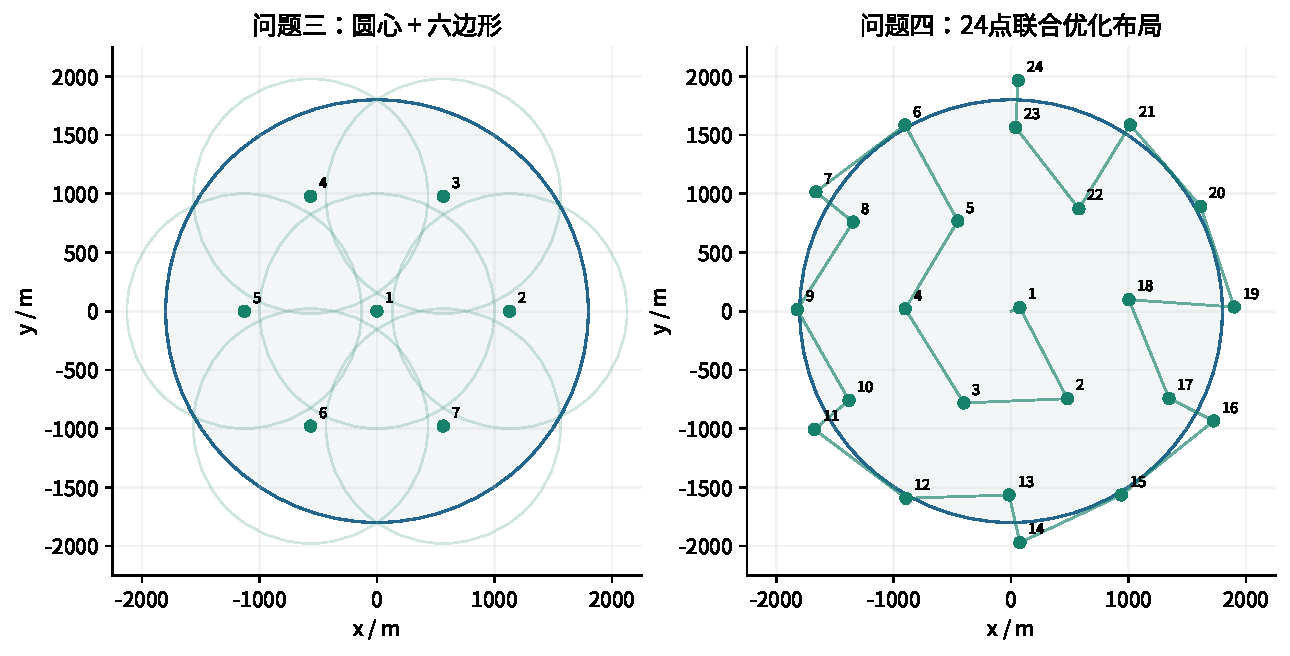
\includegraphics[width=.93\linewidth]{figures/layouts.pdf}
\caption{最终发现层布局：左为问题三七点布局，右为问题四24点布局及离线参考访问顺序。圆外扫描点符合题设移动范围。}\label{fig:layouts}\end{figure}

\subsection{扫描与清除任务联合调度}
固定“先扫描、再逐源清除”会重复经过相邻区域。为此构造动态任务集
\begin{equation}
\mathcal T_t=\{(\mathrm{scan},i,q_i):i\text{尚未访问}\}
\cup\{(\mathrm{clear},j,\widehat G_j):j\text{已发现且未清除}\}.
\end{equation}
只需一条有效读数即可生成目标锚点并登记清除任务。该任务会进一步测量或试清，并不意味着一条读数已经完成定位。

以当前位置为起点，用最近邻构造开放路线，再用2-opt反转片段消除绕行，最后用or-opt将连续1至3个任务搬移至其他位置，接受整条路线长度严格下降的候选，最多执行4轮or-opt。形式上求可行近似解
\begin{equation}
\min_\pi\left\{\norm{z_0-z_{\pi(1)}}+
\sum_{k=1}^{m-1}\norm{z_{\pi(k+1)}-z_{\pi(k)}}\right\},
\end{equation}
其中 $z_0$ 为当前位置。只执行路线首个任务，获得新反馈后重建任务集。这是滚动优化，所得路线是可行上界而非全局最优解；锚点变化使任务实际成本与静态路长不同。

\subsection{直接试清、补测与覆盖式清除}
到达估计点后先尝试光学清除。$r_*(\widehat K_j)>20$ 只表示不能保证该点覆盖全部可能位置，并不表示该点距真源必超过20米。因此以3秒失败代价换取直接命中的机会有实际价值。清除失败后先检查小规模覆盖计划，若不划算，再按问题二的交会原则补测；近共线情况下采用侧向候选。基类补测仍失败时启动覆盖兜底。

将平面划分为边长 $s=25$ 米的方格，格心记为 $z_C$，选择
\begin{equation}
\mathcal H_j=\{C:C\cap\widehat K_j\ne\varnothing\}.
\label{eq:coverclear}
\end{equation}
程序将格网原点对齐至可行域包围盒下界，通过顶点包含与边相交判定选出相交格，减少窄区域的冗余候选。若一个格的四个顶点均位于同一个失败清除圆内，则剔除该格。对其余格心依次试清，命中即停止。
\begin{proposition}
若 $G_j\in\widehat K_j$、清除反馈准确、所选格心均可达且计划完整执行，则覆盖式清除必能清除该目标。
\end{proposition}
\begin{proof}
真源所属方格 $C_G$ 满足 $\norm{z_{C_G}-G_j}\le25/\sqrt2\approx17.678<20$，因而必被选入。由范数凸性，四角均在失败排除圆内意味着整格在圆内，所以含真值的格不会被安全剔除。访问 $z_{C_G}$ 时必能清除目标。
\end{proof}

若计划有 $k$ 个点、全部访问路程为 $L_H$，成功前的最坏耗时上界为
\begin{equation}
T_H\le L_H/5+3k+2.\label{eq:clearcost}
\end{equation}
与“补测再清除”的参考成本 $L_m/5+10+\sigma$ 比较，其中 $\sigma\in\{0,1\}$ 表示是否切频。当前代码采用 $\sigma=1$ 的固定参考，且 $L_m$ 只估计到补测点的移动，所以这是动作选择代理，不是任意反馈下的严格最优判据。固定动作项在 $k=1,2$ 时为5、8秒，均小于10至11秒；$k=3$ 时为11秒，需要结合切频和路程判断。问题三前置计划最多2点，后置最多64点；超过上限时不截取不完整计划冒充覆盖。
\begin{figure}[htbp]\centering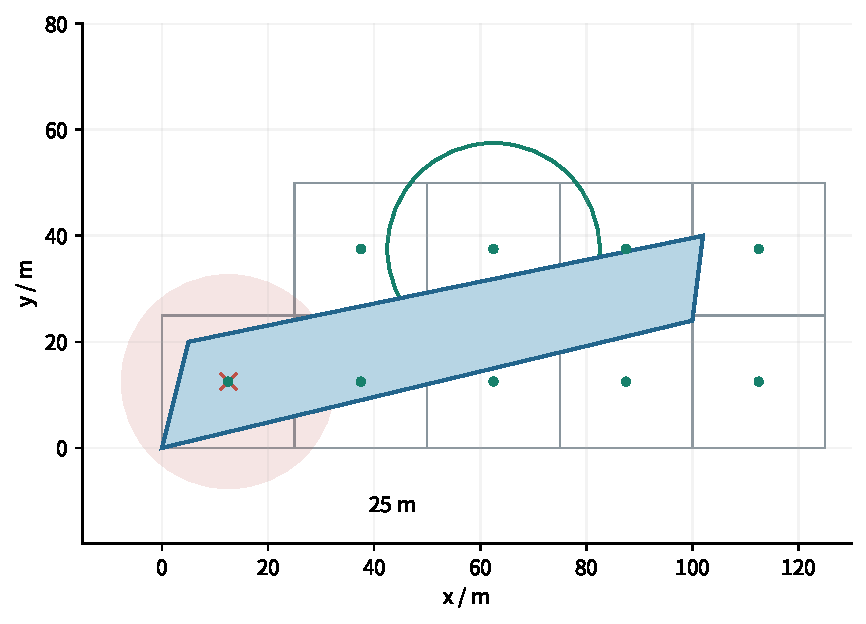
\includegraphics[width=.78\linewidth]{figures/cover_clear.pdf}
\caption{25米方格覆盖式清除示意。蓝色为保守可行域，红色圆为已失败的20米清除范围，绿色圆显示一个格心的有效清除范围。图为几何示意，非真实案例轨迹。}\end{figure}

\subsection{完整流程与保证边界}
\begin{enumerate}
\item 从原点、频道1初始化20个频道状态、知识矩阵及七点扫描任务。
\item 对待扫描点和已发现目标联合规划，每次执行首个任务，按实际反馈更新证据。
\item 执行直接试清、小规模覆盖计划、必要补测和后置覆盖计划，收到成功反馈才移除目标。
\item 扫描任务结束后处理仍未清除频道，核对未知频道的完整扫描记录。
\end{enumerate}
理论上的完成条件是已发现频道全部清除，且每个未发现频道满足
\begin{equation}
\Omega\subseteq\bigcup_{q\in\mathcal N_j}\disk(q,1000).\label{eq:certificate}
\end{equation}
不能以“已清除10个”或“待办队列为空”代替该条件。

上述发现覆盖和清除覆盖均为充分条件，但当前程序还含时间预算、调度重试次数、64格上限及退化区域分支。因此其完整性论证以这些条件未中断覆盖执行为前提，有限批实验的全清率不能提升为所有输入下的无条件保证。若仍有未清目标，需如实报告未完成。对单次示向的1500米长窄扇形，附录给出至多225格的理论兜底构造；该构造可说明有限光学覆盖的存在性，不冒充已接入的64格执行流程。

\section{问题四：混合干扰源的半圆覆盖与自适应清除}
\subsection{定向反馈的联合约束}
设定向源方向为单位向量 $n$。在检测点 $S$ 收到信号的条件为
\begin{equation}
\norm{S-G}\le\rho,\qquad n^\mathsf T(S-G)\ge0.
\end{equation}
定向无信号的含义是
\begin{equation}
\norm{S-G}>\rho\quad\lor\quad n^\mathsf T(S-G)<0.\label{eq:q4negative}
\end{equation}
所以第三问的1000米无线电排除圆不能直接用于混合场景。可以在 $(G,\rho,n)$ 的联合状态中保留该析取，再投影至位置空间；最终实现以正观测的楔形和1500米圆盘维护保守位置域，避免把定向背面误判成距离过远。光学清除与朝向无关，因此20米失败清除圆仍可直接使用。

\subsection{任意朝向发现的局部凸包判据}
令有限检测点集为 $P$，对任意位置 $x\in\Omega$ 定义近邻集合 $P_x=P\cap\disk(x,1000)$。保证未知方向、未知半径的定向源被发现，等价于
\begin{equation}
\boxed{\forall x\in\Omega,\quad x\in\operatorname{conv}(P_x).}\label{eq:localhull}
\end{equation}
\begin{proof}
若 $x$ 是近邻点的凸组合，而某方向 $n$ 对所有近邻均满足 $n^\mathsf T(q-x)<0$，将这些不等式作同一凸组合便得到 $0<0$，矛盾。因此每个闭半圆必有一个可接收检测点。反之，若 $x$ 不属于非空有限近邻集的凸包，严格分离定理给出使全部近邻处于背面的方向；若近邻集为空则显然不能发现。
\end{proof}
该判据同时适用于全向源，且不需要事先识别源的类型。与问题三相比，仅有圆盘并集覆盖不足以满足未知朝向的要求。

\subsection{24点联合优化布局及连续单元证书}
最终 \texttt{q4-v18} 继承24个离线优化检测点，坐标见支撑材料 \texttt{strategy\_v17.py}。优化目标将开放路长与停点检测成本结合：
\begin{equation}
\min_{P,\pi}\ \frac{L(P,\pi)}5+\sum_i(5m_i+s_i),
\quad\text{满足式}\eqref{eq:localhull},
\end{equation}
其中 $m_i$、$s_i$ 是离线阶段对检测数和切频数的估计，实际在线成本由反馈决定。归档布局生成采用软最小值罚函数、L-BFGS-B坐标搜索、几何修复、可行性微调与访问顺序搜索，交替调整坐标和顺序。它是非凸启发式优化，不宣称全局最优，也不将其称为已实现的精确二阶锥规划。

24点的给定离线开放路线为18507.5米。在线仍与清除任务联合调度，故实际路线通常不同，这个数字只用于展示发现布局。

用目标圆包围方形的递归四分构造连续单元证书。对与目标圆相交的方格 $C$，取
\begin{equation}
P_C=\{q\in P:\max_{v\in\operatorname{Vert}(C)}\norm{q-v}\le1000-\tau\}.
\end{equation}
若四个顶点均在 $\operatorname{conv}(P_C)$ 内，则由凸性，整个格内任意 $x$ 都在该凸包中；同时 $P_C\subseteq P_x$，因此整个单元满足式\eqref{eq:localhull}。未通过的单元继续四分；细分到最小边长仍未通过则报告未决，不能当作已覆盖。

现有证书使用 $\tau=10^{-7}$ 米、最小边长0.02米，对24点布局检查3107个相交单元，1992个直接通过，未决单元为0。检查数含中间父单元，不能将3107解释为互不相交叶格数。这是带向内余量的浮点连续区域数值证书，未采用区间算术形式化验证；有限朝向抽样仅作交叉检验。

\subsection{在线精定位与清除}
扫描层保留所有待访问布局点，对未发现频道继续扫描。目标被发现后加入清除任务，滚动最近邻与2-opt统一安排扫描和清除。当前第四问调度继承其独立父类，并未复用第三问的or-opt开关。

精定位先移动至估计点尝试清除，失败后检查最多3点的覆盖计划。若区域仍宽，沿最近一次有效示向的射线分段推进以缩短距离；默认区域直径超过100米时启用，最多12步，单步上限450米。新的有效读数更新保守区域，近距反馈立即清除。无信号可能来自背面，射线上的距离区间仅用于局部搜索调度，不得作为真源的可靠上界。

补测、射线搜索及半径15米六点环形试清均属于启发式。中心加15米六点环只能保证覆盖至约31.53米的估计误差，无法覆盖任意35至40米误差。因此最终在这些流程失败后，针对原保守可行域构造25米格覆盖兜底，并使用所有仍保留的20米失败圆排除整格。由问题三的覆盖命题，该兜底与源朝向无关。

\subsection{结束条件与异常解释}
混合场景完成要求：所有已发现源均收到清除成功反馈，且每个未发现频道实际检测过的点集满足局部凸包覆盖条件。若完整访问24点布局且未知频道均被扫描，后一个条件由离线证书承担；成功清除的频道无需继续检测。

当前实现仍受64格、预算及重试次数上限限制。若计划因上限无法生成，或完整执行后仍未命中，分别表示覆盖流程未完成或保守域前提需要检查，不能把无信号简单解释为目标已消失。第四问的主要改进是将“发现覆盖”和“清除覆盖”分开论证，使波束背面造成的精定位困难最终由与方向无关的光学覆盖处理。

\section{模型检验与实验结果}
\subsection{数据来源与统计口径}
对单案例定义 $\eta=N_c/N_{\rm true}$、$\bar t=T/N_c$，其中 $N_c=0$ 时每源时间未定义，应记录失败。源总数只在测试结束后用于评价，不作为策略的在线输入。跨案例报告全清案例数及逐案例 $\bar t$ 的中位数，不能用 $\sum T/\sum N_c$ 替代该中位数。

本文使用三类证据：最终参数下重新执行的第三问本地消融；仓库保留的第四问逐案例复核JSON及布局证书；官方模拟器两场演练的记录。正式测试另列。旧版失败清除按5秒计算的历史成绩不纳入主表，主表统一使用失败3秒、成功5秒。源位置和方向真值仅用于离线校验。

\subsection{第三问：布局、路由与覆盖清除的消融}
固定模拟器、种子和计时，分别改变布局、or-opt及覆盖清除。布局记为“环顶点数/环半径/每频道扫描读数上限”。各臂在三个种子集上均全清，结果见表\ref{tab:q3ablation}。种子1至30是1至60的子集，不能将两组样本量相加视为独立案例。
\begin{table}[htbp]\centering\small
\caption{第三问最终配置消融：每源时间中位数（秒/源）}\label{tab:q3ablation}
\begin{tabular}{lrrr}\toprule
方法&种子1--30&种子1--60&种子61--160\\\midrule
v8基线&265.92&278.10&278.02\\
v15旧布局，or-opt关&272.41&281.94&279.29\\
v15最终布局，or-opt关&263.81&277.46&278.74\\
v15最终布局，or-opt开&256.68&275.51&271.65\\
v18最终布局，or-opt关&263.24&277.45&278.74\\
v18最终版&256.11&275.54&272.08\\
\bottomrule\end{tabular}
\end{table}
固定or-opt关闭时，布局从7/1110/2改为6/1130/3，三组分别降低8.60、4.48、0.55秒/源；固定最终布局时，开启or-opt分别降低7.13、1.95、7.09秒/源。可见布局收益随案例集变化，不能把不同因素合并归因。

在已开启or-opt的条件下，覆盖式清除相对上一臂的变化为 $-0.57,+0.03,+0.43$ 秒/源，接近中性。采用统一覆盖机制主要为了清除可靠性，而非宣称其在全向场景显著加速。种子61至160中，最终版相对v8的每源时间中位数下降约2.13\%；这是中位数之间的比较，不代表每个案例均下降2.13\%。

\subsection{第四问：发现与清除可靠性}
对默认混合与全定向压力场景，分别使用三个互不重叠的种子段。v14采用较早发现与射线清除机制，v17换成24点布局并增加小环试清，v18增加知识矩阵失败圆与覆盖清除。各方法在同一场景、同一种子下使用相同源配置。
\begin{table}[htbp]\centering\small
\caption{第四问全清案例数与最终版每源时间中位数}\label{tab:q4audit}
\begin{tabular}{llrrrr}\toprule
种子段&场景&v14&v17&v18&v18秒/源\\\midrule
1--60&混合&57/60&60/60&60/60&487.24\\
1--60&全定向&53/60&57/60&60/60&580.73\\
61--160&混合&94/100&97/100&100/100&488.75\\
61--160&全定向&85/100&97/100&100/100&560.44\\
161--260&混合&95/100&98/100&100/100&486.13\\
161--260&全定向&86/100&96/100&100/100&553.15\\
合计&两场景&470/520&505/520&520/520&---\\
\bottomrule\end{tabular}
\end{table}
最终版在520个本地案例中清除6684/6684个源。v17共505/520局全清，v18补齐其15个未全清案例。两个场景复用种子编号，但场景的发射方向构成不同，因此这里计为520个“种子与场景”的组合，不能解释为520次官方测试。

失败记录揭示修复对象：混合场景种子80、频道19的估计误差约33.3米，旧六点环最近试清点仍距真源21.51米；全定向种子128、频道11曾在距真源15.9米处因波束背面返回无信号，射线距离判断随后偏离。二者均已被发现，说明发现完备不等于清除完备。25米格覆盖使用原保守域和方向无关的失败圆，针对这一问题提供最终补救。
\begin{figure}[htbp]\centering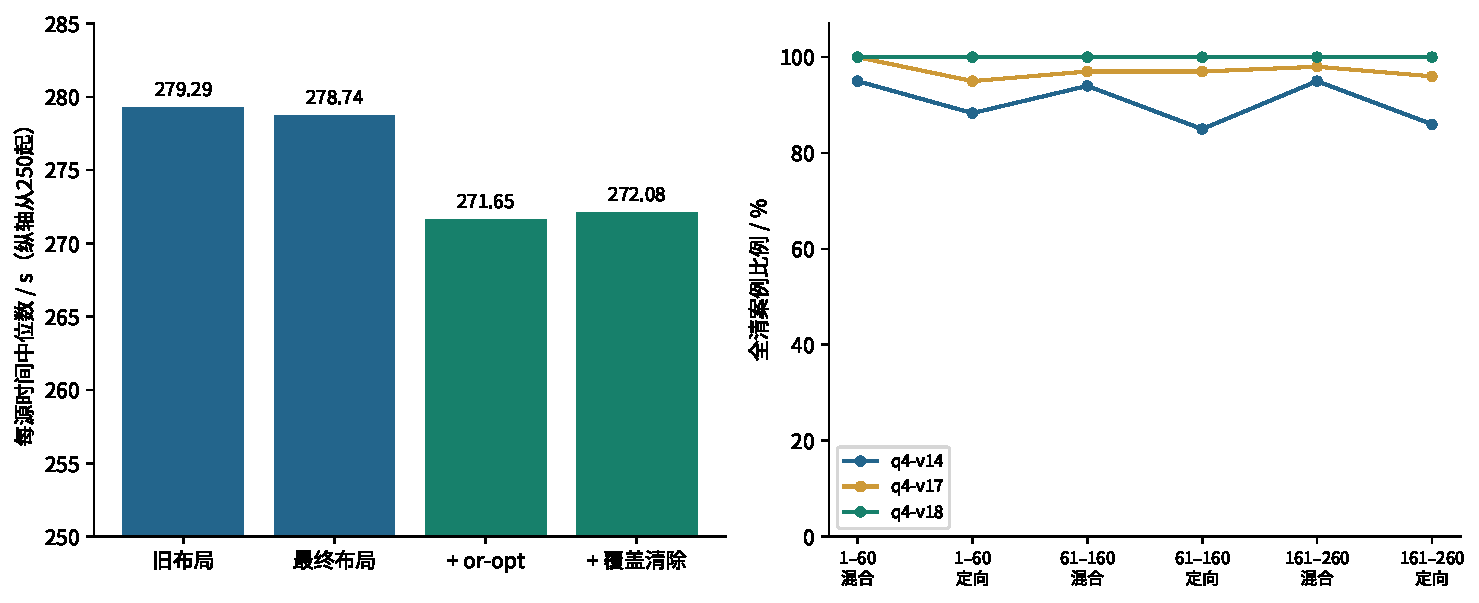
\includegraphics[width=.96\linewidth]{figures/ablation.pdf}
\caption{左：第三问种子61至160的消融；右：第四问六组场景的全清比例。图表来自本地模拟记录。}\end{figure}

\subsection{官方模拟器演练}
2026年9月13日14:19至14:23的两局演练分别使用最终入口 \texttt{q3-v18}、\texttt{q4-v18}，结果记录于支撑材料 \texttt{official-drill-20260913-1420-q18.json}。源总数来自官方测试结束后的结果记录；问题四包含4个全向源及11个定向源。
\begin{table}[htbp]\centering\small
\caption{官方演练结果（每问一场，非正式测试）}
\begin{tabular}{lrr}\toprule
指标&问题三&问题四\\\midrule
案例编码&\texttt{VSSN-5G4G-AWMY-2ENJ}&\texttt{2FAE-SPSW-TG7E-UQH3}\\
清除个数/总数&14/14&15/15\\
清除比例&100\%&100\%\\
虚拟总时间（秒）&3357.525&6339.556\\
平均定位清除时间（秒/源）&239.82&422.64\\
检测次数&110&240\\
清除尝试次数（失败次数）&19（5）&16（1）\\
记录的程序运行时间（秒）&0.5&0.6\\\bottomrule
\end{tabular}\end{table}
两场演练支持最终程序在官方环境中可运行且在对应案例中全清。每问只有一个案例，不能估计稳定的成功率或断言优于另一策略；程序运行时间按现有记录精度保留。官方案例分布、通信和计时环境与本地模拟不同，不直接合并统计。
\placeholder{官方演练代表性轨迹与结果界面}{补充上述两场官方演练的轨迹或Q2回放界面截图，保留案例编码，标出扫描停点、清除位置、虚拟时间和最终清除个数。使用真实导出或回放，不将几何示意图当作实测轨迹。}

\subsection{问题三正式测试结果}
\begin{table}[htbp]\centering\small
\caption{问题三正式测试结果}
\begin{tabular}{llll}\toprule
测试案例编码&清除干扰源个数&平均定位清除时间&程序运行时间\\\midrule
{[正式测试1编码]}&[待填]&[待填，秒/源]&[待填，秒]\\
{[正式测试2编码]}&[待填]&[待填，秒/源]&[待填，秒]\\
{[正式测试3编码]}&[待填]&[待填，秒/源]&[待填，秒]\\\bottomrule
\end{tabular}\end{table}
\subsection{问题四正式测试结果}
\begin{table}[htbp]\centering\small
\caption{问题四正式测试结果}
\begin{tabular}{llll}\toprule
测试案例编码&清除干扰源个数&平均定位清除时间&程序运行时间\\\midrule
{[正式测试1编码]}&[待填]&[待填，秒/源]&[待填，秒]\\
{[正式测试2编码]}&[待填]&[待填，秒/源]&[待填，秒]\\
{[正式测试3编码]}&[待填]&[待填，秒/源]&[待填，秒]\\\bottomrule
\end{tabular}\end{table}
[按每问三次正式测试的官方结果填写以上两表，并将六份官方导出日志以原文件名放入支撑材料。当前可核验记录为演练，不替代正式结果。]

\section{模型评价与改进方向}
本模型将不确定位置表示为可行集，使测向误差界直接参与定位，并区分直径与包围半径。知识矩阵使多类反馈可追溯，联合调度减少扫描与清除的重复移动；局部凸包判据将未知朝向的半圆发现转化为有限几何检验；覆盖式清除利用与方向无关的光学反馈弥补定向背面难题。

模型仍有三方面边界。其一，滚动路由和估计点试清属于启发式，不保证全局最短耗时，负观测修正质心也不保证每个案例都更快。其二，数值外包络、凸包容差及退化区域会影响实现，连续单元证书尚非区间算术证明。其三，64格和执行预算使理论覆盖命题具有执行前提，当前全清结果只能说明所测案例成功，不能消除所有未测情形的风险。

后续可在保持保守域的前提下，对未完成覆盖计划分批续接，保留更完整的负证据事件表，并以同分布、多场官方演练评估稳定性。对当前交付而言，报告实际成功反馈、保存原始日志、区分本地与官方统计，是保证结论可核验的必要条件。

\begin{thebibliography}{9}
\bibitem{problem} 2026年高教社杯全国大学生数学建模竞赛B题：无线电干扰源的快速自动定位与清除（题目及附录1--4）.
\bibitem{protocol} B题附件1：模拟器通信协议与操作说明；附件2：通信示例.
\end{thebibliography}
\clearpage\appendix
\section{几何与概率公式推导}
\subsection{凸多边形直径在顶点对上取得}
设 $X=\sum_i\lambda_iV_i$、$Y=\sum_j\mu_jV_j$，其中系数非负且分别和为1。则
\begin{equation}
\norm{X-Y}=\left\lVert\sum_{i,j}\lambda_i\mu_j(V_i-V_j)\right\rVert
\le\sum_{i,j}\lambda_i\mu_j\norm{V_i-V_j}
\le\max_{i,j}\norm{V_i-V_j}.
\end{equation}
反之，顶点属于多边形，最大顶点距离必能取到，故式\eqref{eq:diameter}成立。圆盘是凸集，所以全部顶点在圆内等价于整个凸多边形在圆内。

\subsection{最小包围圆半径与直径的关系}
包含一对距离为 $D$ 的点需要半径至少 $D/2$。最小包围圆的圆心处于支撑点的凸包内，否则可稍移圆心使所有支撑距离同时减少。在平面上，圆心可由至多三个支撑点的凸组合表示。

两支撑点时，它们为对径点，$r_*=D/2$。三支撑点时，形成包含圆心的三角形，其最大角 $\gamma$ 位于 $[60^\circ,90^\circ]$，由正弦定理最大边长为 $2r_*\sin\gamma\ge\sqrt3r_*$。由于该边不超过 $D$，故 $r_*\le D/\sqrt3$，等边三角形取等号。

三点 $A=(a_x,a_y),B=(b_x,b_y),C=(c_x,c_y)$ 的外接圆心 $U$ 可由
\begin{equation}
2\begin{pmatrix}b_x-a_x&b_y-a_y\\c_x-a_x&c_y-a_y\end{pmatrix}U
=\begin{pmatrix}\norm B^2-\norm A^2\\\norm C^2-\norm A^2\end{pmatrix}
\end{equation}
求解。行列式接近零时应改查最远点对，避免除以近零数。求得圆心后，认证半径统一重算为 $\max_i\norm{U-V_i}$。

\subsection{圆盘外包络的误差}
半径 $r$ 的圆，其外接正 $m$ 边形顶点半径为 $r\sec(\pi/m)$，最大径向外扩为
\begin{equation}
\Delta_m=r\bigl(\sec(\pi/m)-1\bigr)
\simeq\frac{r\pi^2}{2m^2}.
\end{equation}
例如 $r=1800,m=96$ 时约为 $0.964\,\mathrm m$。外包络包含真值，故对它认证清除是保守的；但接近20米阈值时可增加边数或局部精确处理圆弧。该径向外扩不能直接作为任意近乎平行交会后的最终直径误差界，交会几何可能放大误差。

\subsection{三圆交保证区域的证明}
平移旋转后令 $S_1=0,\theta_1=0$，候选点记为向量 $s$，$u_\pm=e(\pm\eps)$。若 $s\in\mathcal V_0$，则
\begin{equation}
\norm s\le a,\qquad \norm{s-au_\pm}\le a
\ \Longrightarrow\ s\cdot u_\pm\ge\frac{\norm s^2}{2a}.
\end{equation}
对 $|\phi|\le\eps$，有 $e(\phi)=\lambda u_-+\mu u_+$，其中
\begin{equation}
\lambda=\frac{\sin(\eps-\phi)}{\sin(2\eps)},\quad
\mu=\frac{\sin(\eps+\phi)}{\sin(2\eps)},\quad
\lambda+\mu=\frac{\cos\phi}{\cos\eps}\ge1.
\end{equation}
故 $s\cdot e(\phi)\ge\norm s^2/(2a)$，进而 $\norm{s-ae(\phi)}\le a$。当 $0\le r\le a$，$re(\phi)$ 是 $0$ 与 $ae(\phi)$ 的凸组合，由距离凸性得 $\norm{s-re(\phi)}\le a$。当 $a\le r\le b$，
\begin{equation}
\norm{s-re(\phi)}^2-r^2
=\norm s^2-2r\,s\cdot e(\phi)
\le\norm s^2(1-r/a)\le0.
\end{equation}
两段分别得到 $d_2\le a$ 与 $d_2\le r$，故总有 $d_2\le\max(a,r)\le\rho$。

完整扇形模型中，取可能源位置 $0,au_-,au_+$ 和半径 $a$，可分别推出三个圆盘约束的必要性。若严格排除 $r\le5$ 或裁去圆域外区域，则这些测试位置可能不再允许，所以此时只保留充分性结论。这个证明也避免了把圆弧扇形的极点误写成只有三个点。

\subsection{径向后验及第二次接收概率}
固定源位置 $G$ 时，允许的接收半径区间是 $[\max(a,d_1),b]$，其长度即 $K_1(d_1)$。两次接收共用半径，所以同时允许的区间长度为 $K_{12}(d_1,d_2)$。这证明式\eqref{eq:weights}，也说明为何不能将两个独立半径的权重相乘。

对圆心第一点，交换积分顺序得
\begin{align}
I_1&=\int_a^b\int_0^\rho r\,\mathrm dr\,\mathrm d\rho
=\frac{b^3-a^3}{6},\\
I_2&=\int_a^b\int_0^\rho r^2\,\mathrm dr\,\mathrm d\rho
=\frac{b^4-a^4}{12}.
\end{align}
严格排除5米近距区后，分母、分子分别变为 $I_1-(b-a)5^2/2$ 与 $I_2-(b-a)5^3/3$。

给定候选点 $S$ 和第二误差 $\delta\in[-\eps,\eps]$，令 $\theta_2=\arg(G-S)+\delta$。任意区域指标 $H$ 的第二次示向条件期望为
\begin{equation}
\mathbb E[H\mid\text{第二次示向}]=
\frac{\displaystyle\int\!\int rK_{12}\ind_{d_2>5}
\left[\frac1{2\eps}\int_{-\eps}^{\eps}H(K_2(S,\theta_2))\,\mathrm d\delta\right]\mathrm dr\,\mathrm d\phi}
{\displaystyle\int\!\int rK_{12}\ind_{d_2>5}\,\mathrm dr\,\mathrm d\phi}.
\end{equation}
严格按第一读数为示向时，径向积分从5开始。取 $H=r_*$ 得平均包围半径，取 $H=\ind_{r_*\le20}$ 得示向条件下的一次认证清除概率；近距分支另加其概率。

对一维积分 $\int_l^u f(t)\,\mathrm dt$，Gauss--Legendre求积写为
\begin{equation}
\int_l^u f(t)\,\mathrm dt\approx\frac{u-l}{2}\sum_{k=1}^q w_k
f\left(\frac{u+l}{2}+\frac{u-l}{2}\xi_k\right).
\end{equation}
将径向、角度和第二误差分别离散，形成张量求积。先在 $r=a$、$d_2=a,b,5$ 及圆域边界处划分区间，能减轻折点影响。确定性求积仍有离散误差，不应称为解析精确值；用加倍节点数比较收敛，并与独立抽样对照。

\subsection{局部交会面积与直径}
取两个单位法向夹角为 $\alpha$，误差带满足 $|n_1\cdot\Delta|\le h_1$、$|n_2\cdot\Delta|\le h_2$。线性映射 $\Delta\mapsto(n_1\cdot\Delta,n_2\cdot\Delta)$ 的行列式绝对值为 $|\sin\alpha|$，故面积为 $4h_1h_2/|\sin\alpha|$。

选 $n_1=(1,0)$、$n_2=(\cos\alpha,\sin\alpha)$，四个顶点为
\begin{equation}
\Delta_{s,t}=\left(s h_1,\frac{t h_2-s h_1\cos\alpha}{\sin\alpha}\right),\qquad s,t\in\{-1,1\}.
\end{equation}
区域中心对称，直径等于最大顶点范数的两倍；选择 $st$ 使交叉项为正即得式\eqref{eq:linear-diameter}。

\subsection{一般正多边形布局的覆盖半径}
设圆心加半径 $r_h\le R_0$ 的正 $n$ 边形顶点，$n\ge3$，令 $\beta=\pi/n$。把平面划为相邻顶点的对称扇区。半径为 $t$ 的点，到最近环顶点的最坏距离出现在扇区中线，其平方为
\begin{equation}
g(t)^2=t^2+r_h^2-2tr_h\cos\beta.
\end{equation}
同时圆心距离为 $t$。两者相等于 $t_0=r_h/(2\cos\beta)$。在 $[0,t_0]$ 上，最近扫描点距离不超过 $t_0$；在 $[t_0,R_0]$ 上，$g(t)^2$ 为凸二次函数，其最大值在端点取得。因此
\begin{equation}
\boxed{c_n(r_h)=\max\left\{\frac{r_h}{2\cos(\pi/n)},
\sqrt{R_0^2+r_h^2-2R_0r_h\cos(\pi/n)}\right\}.}
\label{eq:generalcover}
\end{equation}
该式适用于上述 $n\ge3,\ 0<r_h\le R_0$ 条件，内部项不是 $r_h\sin(\pi/n)$。取六边形、环半径1200米，即得基线覆盖半径968.90米；取八边形、环半径1010米，即得 matrix 布局的949.14米。

若要求 $c_n(r_h)\le a$，必须满足
\begin{equation}
R_0\cos\beta-\sqrt{a^2-R_0^2\sin^2\beta}\le r_h
\le R_0\cos\beta+\sqrt{a^2-R_0^2\sin^2\beta},
\end{equation}
同时满足 $r_h\le2a\cos\beta$ 和 $r_h\le R_0$；根号内为负时，该布局无解。六边形下最小可行环半径为
\begin{equation}
r_{h,\min}=900\sqrt3-100\sqrt{19}\approx1122.96\,\mathrm m.
\end{equation}
圆心起步、沿环访问的开放路径长度为 $r_h+2(n-1)r_h\sin(\pi/n)$。以此加上 $(n+1)$ 个停点的检测和切频代价，可以比较同族布局，但不构成所有搜索路径的全局最优性证明。

\subsection{栅格证书应覆盖整个单元}
若正方形单元边长为 $h$、中心为 $z$，则其中任意点到 $z$ 的距离不超过 $h/\sqrt2$。要证明整个单元位于以检测点 $q$ 为圆心的接收圆内，可以检查
\begin{equation}
\norm{q-z}+h/\sqrt2\le a.
\end{equation}
也可检查正方形四个顶点均在圆盘内，因为圆盘是凸集。只检查格心会把边缘未覆盖位置误判为已覆盖。

对联合半径剪枝，记单元 $B$ 到正观测点的最小距离为 $d_i^-(B)$、到负观测点的最大距离为 $d_k^+(B)$。若
\begin{equation}
\max\left(a,\max_i d_i^-(B)\right)>
\min\left(b,\min_k d_k^+(B)\right),
\end{equation}
则整格不存在可行半径，可安全删除；反向不成立，未被删去的格仍可能不可行，应细分而不是直接认定有源。

\subsection{知识矩阵的证据更新与单调性}
设真实位置与半径为 $(G_j,\rho_j)$。对时刻 $t$ 的反馈 $y_t$，按状态表生成约束集 $\mathcal H(y_t,p_t)$，联合知识更新为
\begin{equation}
\mathcal F_j^{t+1}=\mathcal F_j^t\cap\mathcal H(y_t,p_t).
\end{equation}
若反馈符合题设且 $\mathcal F_j^0$ 包含真值，每个新约束也包含真值，故归纳可知真值始终不被删除。与此同时 $\mathcal F_j^{t+1}\subseteq\mathcal F_j^t$，新信息不会扩大真实可行集。

这一性质要求保留全部有效历史。若一个格的最新证据覆盖掉另一真实位置的旧证据，重建集合可能重新扩大；若把光学失败错误转为无信号，甚至可能删除真值。因此紧凑矩阵应作为历史事件的索引和摘要，完整几何证据宜保留为追加记录。整行标记已清除是任务状态更新，不应抹掉用于复盘的历史内容。

\subsection{半径界的安全性与空域检查}
对任意正观测 $p$，因 $G_j\in\widehat K_j$，有
\begin{equation}
\min_{X\in\widehat K_j}\norm{p-X}\le\norm{p-G_j}\le\rho_j.
\end{equation}
对任意无线电负观测 $q$，有
\begin{equation}
\rho_j<\norm{q-G_j}\le\max_{X\in\widehat K_j}\norm{q-X}.
\end{equation}
仅在全向场景，分别取观测的最大下界和最小上界得到
\begin{equation}
L_j=\max\{a,\max_{p\in\mathcal P_j}\min_{X\in\widehat K_j}\norm{p-X}\},\quad
U_j=\min\{b,\min_{q\in\mathcal N_j}\max_{X\in\widehat K_j}\norm{q-X}\}.
\label{eq:radiusbounds}
\end{equation}
定向场景的无线电无信号不能给出上述上界。若算出 $L_j>U_j$，应检查证据、坐标、事件类别及数值误差，不能通过强行截断掩盖矛盾。

例如真实源在 $(30,0)$、接收半径1000米，在原点光学清除失败，但无线电仍可接收。光学失败只排除20米圆，若将它解释为1000米圆内无信号，会直接删去真实源。矩阵统一记录多类反馈，并不意味着各类反馈共享同一种距离约束。

\subsection{位掩码缺口与有限贪心补测}
对每个频道与每个格组成的任务对 $(j,\ell)$，定义待确认有限全集
\begin{equation}
\mathcal E=\{(j,\ell):\ell\in\mathcal U_j\}.
\end{equation}
候选停点 $S$ 可服务其中整格满足接收保证的任务对，记为 $\mathcal E(S)$。若候选集有限，且已经验证 $\mathcal E\subseteq\bigcup_S\mathcal E(S)$，每次选择新增任务数为正的点并实际完成对应频道测量，则未确认任务数至少减少1。因此至多 $|\mathcal E|$ 步，或至多遍历整个有效候选集合，就能消除当前发现缺口。

这是有限性结论，不是最短路径或最少停点定理；动态候选集和有限预算下仍应检查实际剩余缺口。若仅使用格心构造三角网格，则需额外验证整格条件，不能直接套用连续覆盖半径的结论。

在每次真实动作完成后，先更新矩阵，再更新候选格和覆盖格；只登记真正返回反馈的频道。由于预算中断而未执行的后续频道，不能提前加入已确认集合。这样位掩码的零缺口才具有发现层证书意义。

\subsection{首次示向的有限光学覆盖构造}
以首次示向为局部横轴，真源位于 $[0,1500]\times[-1500\sin\eps,1500\sin\eps]$ 中。将该矩形划为75列、3行，每格横向20米、纵向约17.45米，半对角线约13.27米，小于20米。依次访问225个格心，若真实源仍在该区域且无预算中断，必有一次清除成功。该构造说明有限兜底存在；最终程序实际采用当前可行域的25米相交方格，默认至多64格，两者不可混作同一实现。


\section{最终代码与支撑材料}
\subsection{实现入口和可复现性}
最终问题三、四入口分别为 \texttt{q3-v18}、\texttt{q4-v18}，均由 \texttt{versioned.py} 工厂构造，避免直接实例化父类时漏掉最终参数。支撑材料包含当前工作区的Python核心源码快照，原相对路径和SHA-256见 \texttt{code/MANIFEST.md}；完整程序运行仍以仓库框架和依赖为准。
\begin{longtable}{>{\raggedright\arraybackslash\small}p{4.7cm}p{9.1cm}}\toprule
主要文件&用途\\\midrule\endhead
\texttt{geometry.py}&楔形裁剪、圆盘外包络、区域直径及最小包围圆。\\
\texttt{knowledge.py}&频道—路径稀疏矩阵、真实坐标和反馈摘要。\\
\texttt{knowledge\_layer.py}&失败清除排除圆、相交方格、覆盖计划及代价比较。\\
\texttt{strategy\_v15.py}&问题三的负观测估计修正、2-opt与or-opt调度。\\
\texttt{strategy\_v17.py}&问题四24点布局，继承v14射线搜索和在线调度。\\
\texttt{strategy\_v18.py}&两问最终策略，共用知识矩阵和覆盖清除混入模块。\\
\texttt{versioned.py}&交付入口与参数：问题三6/1130/3、or-opt四轮。\\
{\scriptsize\texttt{q3\_or\_opt\_ablation.py}}&固定计时和种子，分离布局、路由和覆盖清除的收益。\\
{\tiny\texttt{verify\_layout\_certificate.py}}&连续单元覆盖证书和有限采样交叉检验。\\
\texttt{make\_assets.py}&按实际数据生成论文SVG/PDF图和实验表。\\\bottomrule
\end{longtable}

\subsection{离线复现实验命令}
在项目根目录执行下列命令；这些命令只访问本地模拟器和文件。
\begin{Verbatim}[fontsize=\scriptsize,frame=single]
python3 script/run.py --strategy q3-v18 --seed 1
python3 script/run.py --strategy q4-v18 --directional --seed 1
python3 script/q3_or_opt_ablation.py --json paper/build/q3-final-ablation.json
python3 script/verify_layout_certificate.py --layout v17
python3 paper/make_assets.py
python3 paper/verify_formulas.py
bash paper/build.sh
\end{Verbatim}
第三问新复跑结果保存在 \texttt{paper/data/q3-final-ablation.json}；第四问已有逐例记录位于 \texttt{logs/audit/}，论文保留其汇总与源文件哈希。演练汇总保存在 \texttt{paper/data/official-drill-q18.json}，不能代替要求提交的正式原名日志。

\subsection{覆盖式清除核心代码摘录}
以下三个函数省略注释与文档字符串，执行语句直接取自当前 \path{knowledge_layer.py}，辅助几何、类型定义和常量见完整快照。相交格不等于仅格心落入区域，整格剔除也不能简化为格心在失败圆内。覆盖保证还要求保守域包含真值、无不可达格和计划实际执行完成。
\lstinputlisting[language=Python]{code/excerpt_cover_clear.py}

\end{document}
